\documentclass[a4paper,11pt]{article}

% Kodovani (cestiny) v dokumentu: utf-8
%\usepackage[cp1250]{inputenc}	% Omezena stredoevropska kodova stranka, pouze MSW.
\usepackage[utf8]{inputenc}	% Doporucujeme pouzivat UTF-8 (unicode).

\usepackage[margin=2cm]{geometry}
\newtoks\jmenopraktika \newtoks\jmeno \newtoks\datum
\newtoks\obor \newtoks\skupina \newtoks\rocnik \newtoks\semestr
\newtoks\cisloulohy \newtoks\jmenoulohy
\newtoks\tlak \newtoks\teplota \newtoks\vlhkost

\jmenopraktika={Fyzikální praktikum 3}
\jmeno={Lukáš Lejdar}
\datum={25. března 2025}
\obor={F}
\skupina={Út 14:00}

\cisloulohy={11}
\jmenoulohy={Operační zesilovač}

%%%%%%%%%%% Uzitecne balicky:
\usepackage[czech]{babel}

\usepackage{graphicx}
\usepackage{amsmath}
\usepackage{xspace}
\usepackage{url}
\usepackage{indentfirst}
\usepackage{wrapfig}
\usepackage{xcolor}
\usepackage{subfig}
\usepackage{subcaption}
\usepackage{enumitem}
\usepackage{tikzsymbols}
\usepackage{newfloat}

\DeclareFloatingEnvironment[fileext=lof]{graph}
\captionsetup[graph]{labelformat=simple, labelsep=colon, name=Graf}

%%%%%% Zamezeni parchantu:
\widowpenalty 10000 \clubpenalty 10000 \displaywidowpenalty 10000
%%%%%% Parametry pro moznost vsazeni vetsiho poctu obrazku na stranku
\setcounter{topnumber}{3}	  % max. pocet floatu nahore (specifikace t)
\setcounter{bottomnumber}{3}	  % max. pocet floatu dole (specifikace b)
\setcounter{totalnumber}{6}	  % max. pocet floatu na strance celkem
\renewcommand\topfraction{0.9}	  % max podil stranky pro floaty nahore
\renewcommand\bottomfraction{0.9} % max podil stranky pro floaty dole
\renewcommand\textfraction{0.1}	  % min podil stranky, ktery musi obsahovat text
\intextsep=8mm \textfloatsep=8mm  %\intextsep pro ulozeni [h] floatu a \textfloatsep pro [b] or [t]

% Tecky za cisly sekci:
\renewcommand{\thesection}{\arabic{section}.}
\renewcommand{\thesubsection}{\thesection\arabic{subsection}.}
% Jednopismenna mezera mezi cislem a nazvem kapitoly:
\makeatletter \def\@seccntformat#1{\csname the#1\endcsname\hspace{1ex}} \makeatother
%
\newcommand{\vsn}[4]{\ensuremath{#1 =} #2(#3)\,#4}
\newcommand{\vrn}[6]{\ensuremath{#1 =} (#2 $\pm$ #3)\,#4 ($p=$ #5\,\%, $\nu=$ #6)}

\newcommand*\circled[1]{\tikz[baseline=(char.base)]{
		\node[shape=circle,draw,inner sep=1pt] (char) {#1};}}

%%%%%%%%%%%%%%%%%%%%%%%%%%%%%%%%%%%%%%%%%%%%%%%%%%%%%%%%%%%%%%%%%%%%%%%%%%%%%%%
% Zacatek dokumentu
%%%%%%%%%%%%%%%%%%%%%%%%%%%%%%%%%%%%%%%%%%%%%%%%%%%%%%%%%%%%%%%%%%%%%%%%%%%%%%%

\begin{document}


{
\begin{center}
\sf 
{\Large Ústav fyziky a technologií plazmatu Přírodovědecké fakulty Masarykovy univerzity} \\
\bigskip
{\huge \bfseries FYZIKÁLNÍ PRAKTIKUM} \\
\bigskip
{\Large \the\jmenopraktika}
\end{center}

\bigskip

\sf
\noindent
\setlength{\arrayrulewidth}{1pt}
\begin{tabular*}{\textwidth}{@{\extracolsep{\fill}} l l}
\large {\bfseries Zpracoval:}  \the\jmeno & \large  {\bfseries Naměřeno:} \the\datum\\[2mm]
\large  {\bfseries Obor:} \the\obor  \hspace{40mm}  {\bfseries Skupina:} \the\skupina %
&\large {\bfseries Testováno:}\\
\\
\hline
\end{tabular*}
}

\bigskip

{
\sf
\noindent \begin{tabular}{p{4cm} p{0.6\textwidth}}
\Large  Úloha č. {\bfseries \the\cisloulohy:} \par
\smallskip
&\Large \bfseries \the\jmenoulohy  \\[2mm]
\end{tabular}
}

\vspace{-10pt}

\section{Úvod}

Operační zesilovač je součástka reprezentovaná diagramem na obrázku 1, která zesiluje rozdíl napětí mezi jeho invertujícím a neinvertujícím vstupem. Je to aktivní součástka, kterou je potřeba napájet, což reprezentují dva volné vstupy pod zesilovačem.

\begin{figure}[htpb]
    \centering
    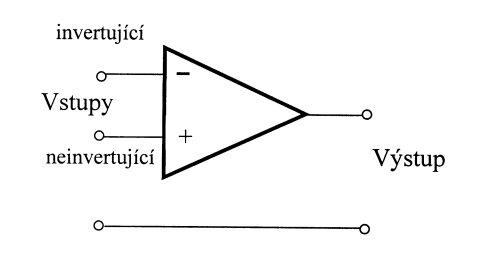
\includegraphics[width=0.35\textwidth]{zesilovac.jpg}
    \caption{Schématická značka operačního zesilovače}
\end{figure}

%Ideální operační zesilovač by měl mít nekonečné zesílení, nekonečný vstupní odpor, nulový výstupní odpor a nekonečnou šířku pásma (tedy zesilovat všechny frekvence stejně). Reálné zesilovače se těmto vlastnostem pouze přibližují - mají vysoké, ale konečné zesílení, vysoký vstupní odpor (řádově $ M \Omega $ ), nízký výstupní odpor (desítky $ \Omega $ ) a omezenou šířku pásma.

Ideální zesilovač má nekonečné zesílení a neteče skrz něj proud. Umí pracovat i se střídavým proudem na vstupu a v takovém případě by měl na všech frekvencích zesilovat stejně. Reálný zesilovač ale funguje dobře jen na nějakém rozmezí. Zavádí se proto pojem šířka pásma, jako ty frekvence při kterých zesílení klesne na nejméně $ A_{u, max} / \sqrt{2}  $  maximální hodnoty. V tomto praktiku ověřím základní vlastnosti zesilovače v několika jednoduchých zapojeních a chování při střídavém signálu na vstupu.

\vspace{20pt}

\section{Měření}

\subsection{Komparátor}

\begin{wrapfigure}[7]{r}{0.4\textwidth}
    \vspace{-30pt}
    \centering
    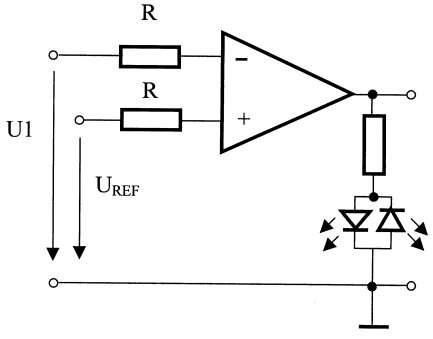
\includegraphics[width=0.3\textwidth]{komparator.jpg}
    \caption{Komparátor}
\end{wrapfigure}

Operační zesilovač jsem zapojil podle obrázku 2 a sledoval která z diod se rozsvítí, jak se mění napětí $ U_1 $  a $ U_\text{ref} $. V případě, že $ U_1 $ bylo větší než $ U_{\text{ref}} $, rozsvítila se dioda propouštějící proud nahoru, tj. na výstupu bylo záporné napětí a v opačném případě kdy polarita byla obrácená svítila druhá dioda. Tímto způsobem se tedy dají binárně porovnávat dvě různé napětí.


%\begin{figure}[h]
%    \centering
%    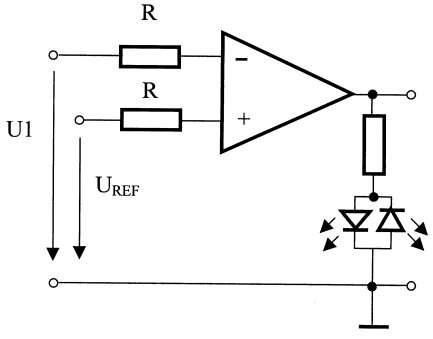
\includegraphics[width=0.3\textwidth]{komparator.jpg}
%    \caption{Komparátor}
%    \vspace{-10pt}
%\end{figure}

\par\noindent

\subsection{Zapojení s invertujícím vstupem}

Schéma zapojení je na obrázku 3, kde smyslem obvodu je zesílit napětí $ U_1 $ o nějaký násobek a obrátit jeho polaritu. K obrácení dochází kvůli zapojení na invertující vstup a zvětšení zajišťuje zpětnovazební rezistor, který uzemní vstup A, takže rezistory $ R_1 $ a $ R_2 $ teče stejný proud.

\begin{equation}
U_{0} = - \frac{R_2}{R_1} U_1
\end{equation}

\begin{figure}[htpb]
    \centering
    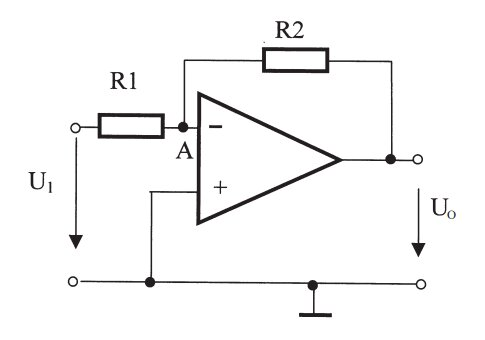
\includegraphics[width=0.4\textwidth]{invertujici_sch.jpg}
    \caption{Zapojení zesilovače s invertujícím vstupem}
\end{figure}

Jako odpory jsem použil $ R_1 = 10 \text{ k} \Omega $ a $ R_2 = 20 \text{ k} \Omega  $ , takže zesílení čekám o velikosti $ - R_2 / R_1 = -2 $. Změřená data pro několik vstupních napětí jsou v tabulce $ 1 $, které jsem nafitoval přímkou pro sklon 

\begin{equation}
\frac{U_0}{U_1} = -2.033 \pm 0.001.
\end{equation}

\begin{table}[h]
    \begin{minipage}{.45\linewidth}
    \vspace{-15pt}
    \centering
    \begin{tabular}{| c c c | }
        \hline
        $ U_1 $ (V) & $ U_0 $ (V) & $ U_0 $ (V)  teoretická \\ \hline
        1.49 & -3.04 & -2.98 \\
        1.76 & -3.58 & -3.52 \\
        1.99 & -4.06 & -3.98 \\
        2.26 & -4.59 & -4.52 \\
        2.47 & -5.02 & -4.94 \\
        2.97 & -6.04 & -5.94 \\
        3.25 & -6.59 & -6.50 \\
        3.48 & -7.08 & -6.96 \\
        3.74 & -7.60 & -7.48 \\
        \hline
    \end{tabular}
    \caption{Naměřené napětí při zapojení s invertujícím vstupem}
    \end{minipage} 
    \hfill
    \begin{minipage}{.5\linewidth}
        \centering
        \resizebox{\textwidth}{!}{ % GNUPLOT: LaTeX picture with Postscript
\begingroup
  \makeatletter
  \providecommand\color[2][]{%
    \GenericError{(gnuplot) \space\space\space\@spaces}{%
      Package color not loaded in conjunction with
      terminal option `colourtext'%
    }{See the gnuplot documentation for explanation.%
    }{Either use 'blacktext' in gnuplot or load the package
      color.sty in LaTeX.}%
    \renewcommand\color[2][]{}%
  }%
  \providecommand\includegraphics[2][]{%
    \GenericError{(gnuplot) \space\space\space\@spaces}{%
      Package graphicx or graphics not loaded%
    }{See the gnuplot documentation for explanation.%
    }{The gnuplot epslatex terminal needs graphicx.sty or graphics.sty.}%
    \renewcommand\includegraphics[2][]{}%
  }%
  \providecommand\rotatebox[2]{#2}%
  \@ifundefined{ifGPcolor}{%
    \newif\ifGPcolor
    \GPcolorfalse
  }{}%
  \@ifundefined{ifGPblacktext}{%
    \newif\ifGPblacktext
    \GPblacktexttrue
  }{}%
  % define a \g@addto@macro without @ in the name:
  \let\gplgaddtomacro\g@addto@macro
  % define empty templates for all commands taking text:
  \gdef\gplbacktext{}%
  \gdef\gplfronttext{}%
  \makeatother
  \ifGPblacktext
    % no textcolor at all
    \def\colorrgb#1{}%
    \def\colorgray#1{}%
  \else
    % gray or color?
    \ifGPcolor
      \def\colorrgb#1{\color[rgb]{#1}}%
      \def\colorgray#1{\color[gray]{#1}}%
      \expandafter\def\csname LTw\endcsname{\color{white}}%
      \expandafter\def\csname LTb\endcsname{\color{black}}%
      \expandafter\def\csname LTa\endcsname{\color{black}}%
      \expandafter\def\csname LT0\endcsname{\color[rgb]{1,0,0}}%
      \expandafter\def\csname LT1\endcsname{\color[rgb]{0,1,0}}%
      \expandafter\def\csname LT2\endcsname{\color[rgb]{0,0,1}}%
      \expandafter\def\csname LT3\endcsname{\color[rgb]{1,0,1}}%
      \expandafter\def\csname LT4\endcsname{\color[rgb]{0,1,1}}%
      \expandafter\def\csname LT5\endcsname{\color[rgb]{1,1,0}}%
      \expandafter\def\csname LT6\endcsname{\color[rgb]{0,0,0}}%
      \expandafter\def\csname LT7\endcsname{\color[rgb]{1,0.3,0}}%
      \expandafter\def\csname LT8\endcsname{\color[rgb]{0.5,0.5,0.5}}%
    \else
      % gray
      \def\colorrgb#1{\color{black}}%
      \def\colorgray#1{\color[gray]{#1}}%
      \expandafter\def\csname LTw\endcsname{\color{white}}%
      \expandafter\def\csname LTb\endcsname{\color{black}}%
      \expandafter\def\csname LTa\endcsname{\color{black}}%
      \expandafter\def\csname LT0\endcsname{\color{black}}%
      \expandafter\def\csname LT1\endcsname{\color{black}}%
      \expandafter\def\csname LT2\endcsname{\color{black}}%
      \expandafter\def\csname LT3\endcsname{\color{black}}%
      \expandafter\def\csname LT4\endcsname{\color{black}}%
      \expandafter\def\csname LT5\endcsname{\color{black}}%
      \expandafter\def\csname LT6\endcsname{\color{black}}%
      \expandafter\def\csname LT7\endcsname{\color{black}}%
      \expandafter\def\csname LT8\endcsname{\color{black}}%
    \fi
  \fi
    \setlength{\unitlength}{0.0500bp}%
    \ifx\gptboxheight\undefined%
      \newlength{\gptboxheight}%
      \newlength{\gptboxwidth}%
      \newsavebox{\gptboxtext}%
    \fi%
    \setlength{\fboxrule}{0.5pt}%
    \setlength{\fboxsep}{1pt}%
    \definecolor{tbcol}{rgb}{1,1,1}%
\begin{picture}(5472.00,3600.00)%
    \gplgaddtomacro\gplbacktext{%
      \csname LTb\endcsname%%
      \put(682,704){\makebox(0,0)[r]{\strut{}$-8$}}%
      \put(682,1190){\makebox(0,0)[r]{\strut{}$-7$}}%
      \put(682,1677){\makebox(0,0)[r]{\strut{}$-6$}}%
      \put(682,2163){\makebox(0,0)[r]{\strut{}$-5$}}%
      \put(682,2649){\makebox(0,0)[r]{\strut{}$-4$}}%
      \put(682,3136){\makebox(0,0)[r]{\strut{}$-3$}}%
      \put(1201,484){\makebox(0,0){\strut{}$1.5$}}%
      \put(1976,484){\makebox(0,0){\strut{}$2$}}%
      \put(2751,484){\makebox(0,0){\strut{}$2.5$}}%
      \put(3526,484){\makebox(0,0){\strut{}$3$}}%
      \put(4300,484){\makebox(0,0){\strut{}$3.5$}}%
      \put(5075,484){\makebox(0,0){\strut{}$4$}}%
    }%
    \gplgaddtomacro\gplfronttext{%
      \csname LTb\endcsname%%
      \put(209,2041){\rotatebox{-270}{\makebox(0,0){\strut{}$ U_0 $ (V) }}}%
      \put(2944,154){\makebox(0,0){\strut{}$ U_1 $ (V)}}%
      \csname LTb\endcsname%%
      \put(4088,3206){\makebox(0,0)[r]{\strut{}fit }}%
    }%
    \gplbacktext
    \put(0,0){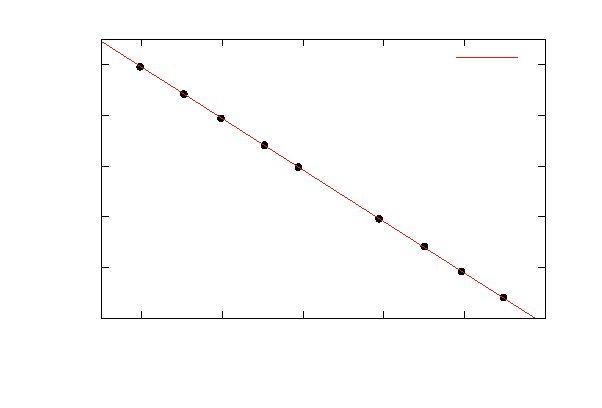
\includegraphics[width={273.60bp},height={180.00bp}]{invertujici}}%
    \gplfronttext
  \end{picture}%
\endgroup
 }
        \captionsetup{type=graph}
        \caption{Závislost výstupního napětí na vstupním při zapojení s invertujícím vstupem}
    \end{minipage} 
\end{table}

\subsection{Šířka pásma zapojení s invertujícím vstupem}

Zapojení nechám stejné, ale tentokrát na vstup přivedu střídavé napětí o frekvenci $ \omega $ a výstup budu měřit osciloskopem. Naměřená data jsou uvedená v tabulce 3 a zesílení $ A_u = U_0 / U_1 $ jsem vynesl do grafu 2. Je vidět, že zesílení si drží hodnotu $ 2 $ až do frekvence vstupu $ \omega = 25 $ kHz a pak postupně klesá k nule. Šířka operačního pásma je tedy rozmezí, kdy hodnoty překračují hodnotu $ A_{u,max} / \sqrt{2} = 2 / \sqrt{2} = \sqrt{2}    $, takže interval $ \omega \in (0, 40) $   kHz.

\newpage

\begin{table}[htpb]
    \begin{minipage}{.45\linewidth}
        \centering
        \begin{tabular}{| c c c c |}
            \hline
            $ \omega $  (kHz) & $ U_0 $ (V) & $ U_1 $ (V) & $ A_u $  \\
            \hline
            00.500 & 4.266 & 2.133 & 2.000 \\
            10.000 & 4.296 & 2.133 & 2.014 \\
            20.000 & 4.297 & 2.133 & 2.015 \\
            25.000 & 4.210 & 2.133 & 1.974 \\
            30.000 & 3.906 & 2.133 & 1.831 \\
            32.000 & 3.600 & 2.133 & 1.688 \\
            34.000 & 3.515 & 2.133 & 1.648 \\
            36.000 & 3.320 & 2.133 & 1.556 \\
            38.000 & 3.125 & 2.133 & 1.465 \\
            40.000 & 3.027 & 2.133 & 1.419 \\
            42.000 & 2.832 & 2.133 & 1.328 \\
            45.000 & 2.637 & 2.133 & 1.236 \\
            47.000 & 2.539 & 2.133 & 1.190 \\
            50.000 & 2.441 & 2.133 & 1.144 \\
            60.000 & 1.953 & 2.133 & 0.916 \\
            \hline
        \end{tabular}
        \caption{Změřené amplitudy napětí střídavého vstupního a výstupního napětí}
    \end{minipage} 
    \hfill
    \begin{minipage}{.45\linewidth}
        \centering
        \resizebox{\textwidth}{!}{ % GNUPLOT: LaTeX picture with Postscript
\begingroup
  \makeatletter
  \providecommand\color[2][]{%
    \GenericError{(gnuplot) \space\space\space\@spaces}{%
      Package color not loaded in conjunction with
      terminal option `colourtext'%
    }{See the gnuplot documentation for explanation.%
    }{Either use 'blacktext' in gnuplot or load the package
      color.sty in LaTeX.}%
    \renewcommand\color[2][]{}%
  }%
  \providecommand\includegraphics[2][]{%
    \GenericError{(gnuplot) \space\space\space\@spaces}{%
      Package graphicx or graphics not loaded%
    }{See the gnuplot documentation for explanation.%
    }{The gnuplot epslatex terminal needs graphicx.sty or graphics.sty.}%
    \renewcommand\includegraphics[2][]{}%
  }%
  \providecommand\rotatebox[2]{#2}%
  \@ifundefined{ifGPcolor}{%
    \newif\ifGPcolor
    \GPcolorfalse
  }{}%
  \@ifundefined{ifGPblacktext}{%
    \newif\ifGPblacktext
    \GPblacktexttrue
  }{}%
  % define a \g@addto@macro without @ in the name:
  \let\gplgaddtomacro\g@addto@macro
  % define empty templates for all commands taking text:
  \gdef\gplbacktext{}%
  \gdef\gplfronttext{}%
  \makeatother
  \ifGPblacktext
    % no textcolor at all
    \def\colorrgb#1{}%
    \def\colorgray#1{}%
  \else
    % gray or color?
    \ifGPcolor
      \def\colorrgb#1{\color[rgb]{#1}}%
      \def\colorgray#1{\color[gray]{#1}}%
      \expandafter\def\csname LTw\endcsname{\color{white}}%
      \expandafter\def\csname LTb\endcsname{\color{black}}%
      \expandafter\def\csname LTa\endcsname{\color{black}}%
      \expandafter\def\csname LT0\endcsname{\color[rgb]{1,0,0}}%
      \expandafter\def\csname LT1\endcsname{\color[rgb]{0,1,0}}%
      \expandafter\def\csname LT2\endcsname{\color[rgb]{0,0,1}}%
      \expandafter\def\csname LT3\endcsname{\color[rgb]{1,0,1}}%
      \expandafter\def\csname LT4\endcsname{\color[rgb]{0,1,1}}%
      \expandafter\def\csname LT5\endcsname{\color[rgb]{1,1,0}}%
      \expandafter\def\csname LT6\endcsname{\color[rgb]{0,0,0}}%
      \expandafter\def\csname LT7\endcsname{\color[rgb]{1,0.3,0}}%
      \expandafter\def\csname LT8\endcsname{\color[rgb]{0.5,0.5,0.5}}%
    \else
      % gray
      \def\colorrgb#1{\color{black}}%
      \def\colorgray#1{\color[gray]{#1}}%
      \expandafter\def\csname LTw\endcsname{\color{white}}%
      \expandafter\def\csname LTb\endcsname{\color{black}}%
      \expandafter\def\csname LTa\endcsname{\color{black}}%
      \expandafter\def\csname LT0\endcsname{\color{black}}%
      \expandafter\def\csname LT1\endcsname{\color{black}}%
      \expandafter\def\csname LT2\endcsname{\color{black}}%
      \expandafter\def\csname LT3\endcsname{\color{black}}%
      \expandafter\def\csname LT4\endcsname{\color{black}}%
      \expandafter\def\csname LT5\endcsname{\color{black}}%
      \expandafter\def\csname LT6\endcsname{\color{black}}%
      \expandafter\def\csname LT7\endcsname{\color{black}}%
      \expandafter\def\csname LT8\endcsname{\color{black}}%
    \fi
  \fi
    \setlength{\unitlength}{0.0500bp}%
    \ifx\gptboxheight\undefined%
      \newlength{\gptboxheight}%
      \newlength{\gptboxwidth}%
      \newsavebox{\gptboxtext}%
    \fi%
    \setlength{\fboxrule}{0.5pt}%
    \setlength{\fboxsep}{1pt}%
    \definecolor{tbcol}{rgb}{1,1,1}%
\begin{picture}(5760.00,4030.00)%
    \gplgaddtomacro\gplbacktext{%
      \csname LTb\endcsname%%
      \put(814,704){\makebox(0,0)[r]{\strut{}$0.8$}}%
      \put(814,1148){\makebox(0,0)[r]{\strut{}$1$}}%
      \put(814,1591){\makebox(0,0)[r]{\strut{}$1.2$}}%
      \put(814,2035){\makebox(0,0)[r]{\strut{}$1.4$}}%
      \put(814,2478){\makebox(0,0)[r]{\strut{}$1.6$}}%
      \put(814,2922){\makebox(0,0)[r]{\strut{}$1.8$}}%
      \put(814,3365){\makebox(0,0)[r]{\strut{}$2$}}%
      \put(814,3809){\makebox(0,0)[r]{\strut{}$2.2$}}%
      \put(946,484){\makebox(0,0){\strut{}$0$}}%
      \put(1682,484){\makebox(0,0){\strut{}$10$}}%
      \put(2418,484){\makebox(0,0){\strut{}$20$}}%
      \put(3155,484){\makebox(0,0){\strut{}$30$}}%
      \put(3891,484){\makebox(0,0){\strut{}$40$}}%
      \put(4627,484){\makebox(0,0){\strut{}$50$}}%
      \put(5363,484){\makebox(0,0){\strut{}$60$}}%
    }%
    \gplgaddtomacro\gplfronttext{%
      \csname LTb\endcsname%%
      \put(209,2256){\rotatebox{-270}{\makebox(0,0){\strut{}$ A_u $}}}%
      \put(3154,154){\makebox(0,0){\strut{}$ f $ (kHz) }}%
      \csname LTb\endcsname%%
      \put(4376,3636){\makebox(0,0)[r]{\strut{}$ A_{u,max} / \sqrt(2) $ }}%
    }%
    \gplbacktext
    \put(0,0){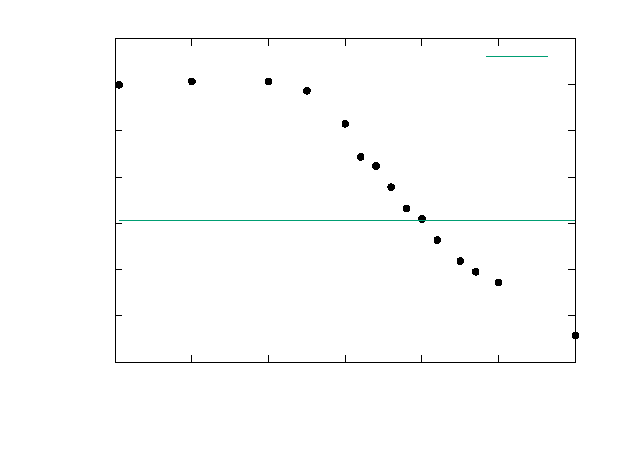
\includegraphics[width={288.00bp},height={201.50bp}]{pasmo}}%
    \gplfronttext
  \end{picture}%
\endgroup
 }
        \captionsetup{type=graph}
        \caption{Závislost zesílení na na frekvenci }
    \end{minipage} 
\end{table}

\subsection{Dolnofrekvenční propust}

Malou změnou zapojení z obrázku 3 na 4 dostaneme zapojení, které propouští pouze nízké frekvence vstupního signálu. Přidaný kondenzátor snižuje impedanci zpětnovazební větve pro vysoké frekvence, což vede k zesílení

\begin{equation}
\frac{U_0}{U_1} = A_u = -\frac{R_F}{R_A} \frac{1}{ \sqrt{1 + \omega^2 C_F^2 R_F^2} } 
\end{equation}

\begin{figure}[h]
    \centering
    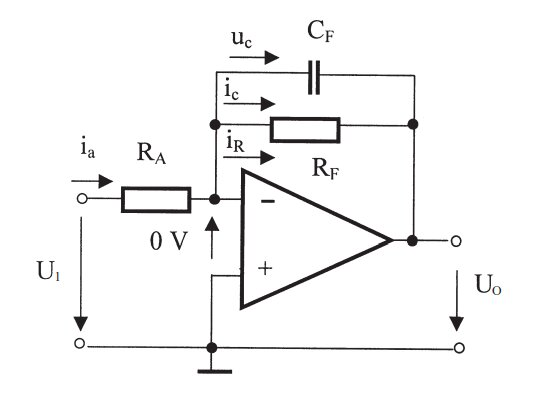
\includegraphics[width=0.4\textwidth]{propust.jpg}
    \caption{Dolnofrekvenční propust}
\end{figure}

Použil jsem kondenzátor o kapacitě $ C_F = 10  $ nF a odpory $ R_F = 100 $ k$\Omega$ a $ R_A = 10 $ k$ \Omega $, takže očekávám maximální zesílení pro $ \omega = 0 $ 

\begin{equation}
A_{\text{u max}} = - 10.0
\end{equation}


Na vstup jsem přivedl střídavé napětí o frekvenci $ \omega $ a stabilní amplitudě $ U_1 = 1.120 $ V a měřil amplitudu výstupního napětí. Naměřená data jsou v tabulce 3 a graf 3 je porovnává s teoretickým vztahem (3). Šířka pásma je v tomto případě $ \omega \in (0, 168) $ kHz.

\begin{table}[h]
    \begin{minipage}{.5\linewidth}
        \centering
        \begin{tabular}{| c c c c c |}
            \hline
            $ \omega $ (kHz) & $ U_1 $ (V)  & $ U_0 $  (V) & $ U_0 $ teorie (V) & $ A_u $  \\
            \hline    
            10  & 1.120 &  -10.898  &  -11.16 & -9.980 \\
            50  & 1.120 &  -10.494  &  -10.67 & -9.540 \\
            80  & 1.120 &  -10.0    &  -9.98  & -8.935 \\
            100 & 1.120 &  -9.28    &  -9.46  & -8.467 \\
            130 & 1.120 &  -8.476   &  -8.65  & -7.744 \\
            150 & 1.120 &  -8.072   &  -8.13  & -7.277 \\
            170 & 1.120 &  -7.669   &  -7.64  & -6.834 \\
            200 & 1.120 &  -7.26    &  -6.96  & -6.226 \\
            220 & 1.120 &  -6.86    &  -6.55  & -5.861 \\
            250 & 1.120 &  -6.054   &  -6.00  & -5.370 \\
            270 & 1.120 &  -5.65    &  -5.67  & -5.078 \\
            300 & 1.120 &  -5.24    &  -5.23  & -4.686 \\
            350 & 1.120 &  -4.84    &  -4.62  & -4.139 \\
            400 & 1.120 &  -4.43    &  -4.13  & -3.696 \\
            500 & 1.120 &  -3.63    &  -3.39  & -3.033 \\
            600 & 1.120 &  -3.229   &  -2.86  & -2.563 \\
            \hline
        \end{tabular}
        \caption{Měření dolnofrekvenční propusti}
    \end{minipage} 
    \hfill
    \begin{minipage}{.45\linewidth}
        \centering
        \resizebox{\textwidth}{!}{ % GNUPLOT: LaTeX picture with Postscript
\begingroup
  \makeatletter
  \providecommand\color[2][]{%
    \GenericError{(gnuplot) \space\space\space\@spaces}{%
      Package color not loaded in conjunction with
      terminal option `colourtext'%
    }{See the gnuplot documentation for explanation.%
    }{Either use 'blacktext' in gnuplot or load the package
      color.sty in LaTeX.}%
    \renewcommand\color[2][]{}%
  }%
  \providecommand\includegraphics[2][]{%
    \GenericError{(gnuplot) \space\space\space\@spaces}{%
      Package graphicx or graphics not loaded%
    }{See the gnuplot documentation for explanation.%
    }{The gnuplot epslatex terminal needs graphicx.sty or graphics.sty.}%
    \renewcommand\includegraphics[2][]{}%
  }%
  \providecommand\rotatebox[2]{#2}%
  \@ifundefined{ifGPcolor}{%
    \newif\ifGPcolor
    \GPcolorfalse
  }{}%
  \@ifundefined{ifGPblacktext}{%
    \newif\ifGPblacktext
    \GPblacktexttrue
  }{}%
  % define a \g@addto@macro without @ in the name:
  \let\gplgaddtomacro\g@addto@macro
  % define empty templates for all commands taking text:
  \gdef\gplbacktext{}%
  \gdef\gplfronttext{}%
  \makeatother
  \ifGPblacktext
    % no textcolor at all
    \def\colorrgb#1{}%
    \def\colorgray#1{}%
  \else
    % gray or color?
    \ifGPcolor
      \def\colorrgb#1{\color[rgb]{#1}}%
      \def\colorgray#1{\color[gray]{#1}}%
      \expandafter\def\csname LTw\endcsname{\color{white}}%
      \expandafter\def\csname LTb\endcsname{\color{black}}%
      \expandafter\def\csname LTa\endcsname{\color{black}}%
      \expandafter\def\csname LT0\endcsname{\color[rgb]{1,0,0}}%
      \expandafter\def\csname LT1\endcsname{\color[rgb]{0,1,0}}%
      \expandafter\def\csname LT2\endcsname{\color[rgb]{0,0,1}}%
      \expandafter\def\csname LT3\endcsname{\color[rgb]{1,0,1}}%
      \expandafter\def\csname LT4\endcsname{\color[rgb]{0,1,1}}%
      \expandafter\def\csname LT5\endcsname{\color[rgb]{1,1,0}}%
      \expandafter\def\csname LT6\endcsname{\color[rgb]{0,0,0}}%
      \expandafter\def\csname LT7\endcsname{\color[rgb]{1,0.3,0}}%
      \expandafter\def\csname LT8\endcsname{\color[rgb]{0.5,0.5,0.5}}%
    \else
      % gray
      \def\colorrgb#1{\color{black}}%
      \def\colorgray#1{\color[gray]{#1}}%
      \expandafter\def\csname LTw\endcsname{\color{white}}%
      \expandafter\def\csname LTb\endcsname{\color{black}}%
      \expandafter\def\csname LTa\endcsname{\color{black}}%
      \expandafter\def\csname LT0\endcsname{\color{black}}%
      \expandafter\def\csname LT1\endcsname{\color{black}}%
      \expandafter\def\csname LT2\endcsname{\color{black}}%
      \expandafter\def\csname LT3\endcsname{\color{black}}%
      \expandafter\def\csname LT4\endcsname{\color{black}}%
      \expandafter\def\csname LT5\endcsname{\color{black}}%
      \expandafter\def\csname LT6\endcsname{\color{black}}%
      \expandafter\def\csname LT7\endcsname{\color{black}}%
      \expandafter\def\csname LT8\endcsname{\color{black}}%
    \fi
  \fi
    \setlength{\unitlength}{0.0500bp}%
    \ifx\gptboxheight\undefined%
      \newlength{\gptboxheight}%
      \newlength{\gptboxwidth}%
      \newsavebox{\gptboxtext}%
    \fi%
    \setlength{\fboxrule}{0.5pt}%
    \setlength{\fboxsep}{1pt}%
    \definecolor{tbcol}{rgb}{1,1,1}%
\begin{picture}(4896.00,3600.00)%
    \gplgaddtomacro\gplbacktext{%
      \csname LTb\endcsname%%
      \put(814,3379){\makebox(0,0)[r]{\strut{}$-12$}}%
      \put(814,2844){\makebox(0,0)[r]{\strut{}$-10$}}%
      \put(814,2309){\makebox(0,0)[r]{\strut{}$-8$}}%
      \put(814,1774){\makebox(0,0)[r]{\strut{}$-6$}}%
      \put(814,1239){\makebox(0,0)[r]{\strut{}$-4$}}%
      \put(814,704){\makebox(0,0)[r]{\strut{}$-2$}}%
      \put(946,484){\makebox(0,0){\strut{}$0$}}%
      \put(1538,484){\makebox(0,0){\strut{}$100$}}%
      \put(2130,484){\makebox(0,0){\strut{}$200$}}%
      \put(2723,484){\makebox(0,0){\strut{}$300$}}%
      \put(3315,484){\makebox(0,0){\strut{}$400$}}%
      \put(3907,484){\makebox(0,0){\strut{}$500$}}%
      \put(4499,484){\makebox(0,0){\strut{}$600$}}%
    }%
    \gplgaddtomacro\gplfronttext{%
      \csname LTb\endcsname%%
      \put(209,2041){\rotatebox{-270}{\makebox(0,0){\strut{}$ A_u $}}}%
      \put(2722,154){\makebox(0,0){\strut{}$ \omega $ (kHz)}}%
      \csname LTb\endcsname%%
      \put(3512,3206){\makebox(0,0)[r]{\strut{}teoretická závislost}}%
      \csname LTb\endcsname%%
      \put(3512,2986){\makebox(0,0)[r]{\strut{}$ A_{u,max} / \sqrt(2) $ }}%
    }%
    \gplbacktext
    \put(0,0){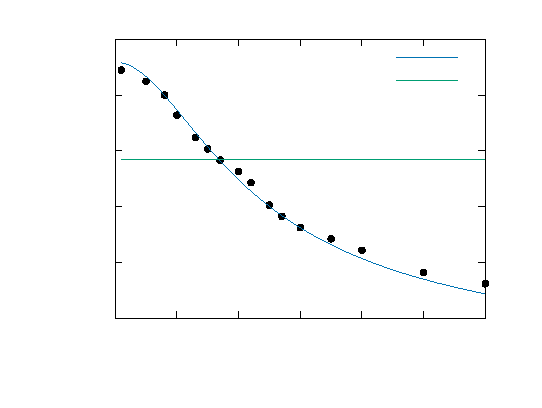
\includegraphics[width={244.80bp},height={180.00bp}]{dolnofrekvencni_propust}}%
    \gplfronttext
  \end{picture}%
\endgroup
 }
        \captionsetup{type=graph}
        \caption{Závislost zesílení na frekvenci vstupního napětí}
    \end{minipage} 
\end{table}

\subsection{Zapojení s neinvertujícím vstupem}

Zapojení je stejné jako při invertujícím, ale napětí $ U_1 $ je tentokrát přivedeme na neinvertující vstup. Obvod se ustálí ve stavu, kdy je na invertujícím vstupu stejné napětí jako na neinvertujícím a pokud proud opět teče jen skrz odpory $ R_1 $ a $ R_2 $, musí platit

\begin{equation}
\frac{U_1}{R_1} = \frac{U_0}{R_1 + R_2}
\end{equation}

\noindent
odkud po úpravě vychází

\begin{equation}
U_0 = \left( 1 + \frac{R_2}{R_1} \right) U_1
\end{equation}


\begin{figure}[h]
    \centering
    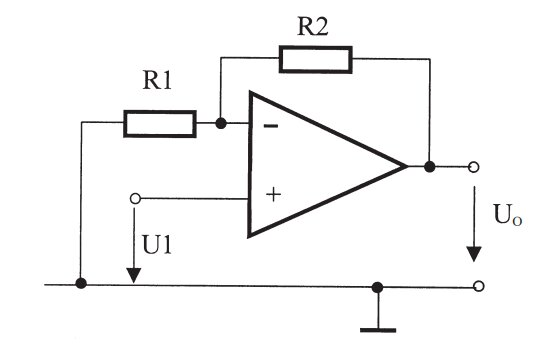
\includegraphics[width=0.4\textwidth]{neinvertujici_sch.jpg}
    \caption{Zapojení neinvertujícího zesilovače}
\end{figure}

Odpory $ R_2 = 20 \text{ k} \Omega $, $ R_1 = 10 \text{ k} \Omega $ zůstali stejné, takže zesílení signálu bude $ R_2 / (R_1 + R_2) = 3 $. Naměřená data jsou v tabulce (3) a fitem přímkou jsem dostal zesílení

\begin{equation}
\frac{U_0}{U_1} = 3.045 \pm 0.002
\end{equation}

\begin{table}[h]
    \begin{minipage}{.45\linewidth}
    \vspace{-15pt}
    \centering
    \begin{tabular}{| c c c | }
        \hline
        $ U_1 $ (V) & $ U_0 $ (V) & $ U_0 $ (V)  teoretická \\ \hline
       1.25 & 3.83  &  3.75  \\
       1.49 & 4.54  &  4.47  \\
       1.76 & 5.37  &  5.28  \\
       1.99 & 6.07  &  5.97  \\
       2.25 & 6.86  &  6.75  \\
       2.50 & 7.61  &  7.5   \\
       2.75 & 8.38  &  8.25  \\
       2.99 & 9.09  &  8.97  \\
       3.26 & 9.91  &  9.78  \\
       3.49 & 10.62 &  10.47 \\
        \hline
    \end{tabular}
    \caption{Naměřené napětí při zapojení s neinvertujícím vstupem}
    \end{minipage} 
    \hfill
    \begin{minipage}{.5\linewidth}
        \centering
        \resizebox{\textwidth}{!}{ % GNUPLOT: LaTeX picture with Postscript
\begingroup
  \makeatletter
  \providecommand\color[2][]{%
    \GenericError{(gnuplot) \space\space\space\@spaces}{%
      Package color not loaded in conjunction with
      terminal option `colourtext'%
    }{See the gnuplot documentation for explanation.%
    }{Either use 'blacktext' in gnuplot or load the package
      color.sty in LaTeX.}%
    \renewcommand\color[2][]{}%
  }%
  \providecommand\includegraphics[2][]{%
    \GenericError{(gnuplot) \space\space\space\@spaces}{%
      Package graphicx or graphics not loaded%
    }{See the gnuplot documentation for explanation.%
    }{The gnuplot epslatex terminal needs graphicx.sty or graphics.sty.}%
    \renewcommand\includegraphics[2][]{}%
  }%
  \providecommand\rotatebox[2]{#2}%
  \@ifundefined{ifGPcolor}{%
    \newif\ifGPcolor
    \GPcolorfalse
  }{}%
  \@ifundefined{ifGPblacktext}{%
    \newif\ifGPblacktext
    \GPblacktexttrue
  }{}%
  % define a \g@addto@macro without @ in the name:
  \let\gplgaddtomacro\g@addto@macro
  % define empty templates for all commands taking text:
  \gdef\gplbacktext{}%
  \gdef\gplfronttext{}%
  \makeatother
  \ifGPblacktext
    % no textcolor at all
    \def\colorrgb#1{}%
    \def\colorgray#1{}%
  \else
    % gray or color?
    \ifGPcolor
      \def\colorrgb#1{\color[rgb]{#1}}%
      \def\colorgray#1{\color[gray]{#1}}%
      \expandafter\def\csname LTw\endcsname{\color{white}}%
      \expandafter\def\csname LTb\endcsname{\color{black}}%
      \expandafter\def\csname LTa\endcsname{\color{black}}%
      \expandafter\def\csname LT0\endcsname{\color[rgb]{1,0,0}}%
      \expandafter\def\csname LT1\endcsname{\color[rgb]{0,1,0}}%
      \expandafter\def\csname LT2\endcsname{\color[rgb]{0,0,1}}%
      \expandafter\def\csname LT3\endcsname{\color[rgb]{1,0,1}}%
      \expandafter\def\csname LT4\endcsname{\color[rgb]{0,1,1}}%
      \expandafter\def\csname LT5\endcsname{\color[rgb]{1,1,0}}%
      \expandafter\def\csname LT6\endcsname{\color[rgb]{0,0,0}}%
      \expandafter\def\csname LT7\endcsname{\color[rgb]{1,0.3,0}}%
      \expandafter\def\csname LT8\endcsname{\color[rgb]{0.5,0.5,0.5}}%
    \else
      % gray
      \def\colorrgb#1{\color{black}}%
      \def\colorgray#1{\color[gray]{#1}}%
      \expandafter\def\csname LTw\endcsname{\color{white}}%
      \expandafter\def\csname LTb\endcsname{\color{black}}%
      \expandafter\def\csname LTa\endcsname{\color{black}}%
      \expandafter\def\csname LT0\endcsname{\color{black}}%
      \expandafter\def\csname LT1\endcsname{\color{black}}%
      \expandafter\def\csname LT2\endcsname{\color{black}}%
      \expandafter\def\csname LT3\endcsname{\color{black}}%
      \expandafter\def\csname LT4\endcsname{\color{black}}%
      \expandafter\def\csname LT5\endcsname{\color{black}}%
      \expandafter\def\csname LT6\endcsname{\color{black}}%
      \expandafter\def\csname LT7\endcsname{\color{black}}%
      \expandafter\def\csname LT8\endcsname{\color{black}}%
    \fi
  \fi
    \setlength{\unitlength}{0.0500bp}%
    \ifx\gptboxheight\undefined%
      \newlength{\gptboxheight}%
      \newlength{\gptboxwidth}%
      \newsavebox{\gptboxtext}%
    \fi%
    \setlength{\fboxrule}{0.5pt}%
    \setlength{\fboxsep}{1pt}%
    \definecolor{tbcol}{rgb}{1,1,1}%
\begin{picture}(5182.00,3168.00)%
    \gplgaddtomacro\gplbacktext{%
      \csname LTb\endcsname%%
      \put(682,704){\makebox(0,0)[r]{\strut{}$3$}}%
      \put(682,953){\makebox(0,0)[r]{\strut{}$4$}}%
      \put(682,1202){\makebox(0,0)[r]{\strut{}$5$}}%
      \put(682,1452){\makebox(0,0)[r]{\strut{}$6$}}%
      \put(682,1701){\makebox(0,0)[r]{\strut{}$7$}}%
      \put(682,1950){\makebox(0,0)[r]{\strut{}$8$}}%
      \put(682,2199){\makebox(0,0)[r]{\strut{}$9$}}%
      \put(682,2449){\makebox(0,0)[r]{\strut{}$10$}}%
      \put(682,2698){\makebox(0,0)[r]{\strut{}$11$}}%
      \put(682,2947){\makebox(0,0)[r]{\strut{}$12$}}%
      \put(814,484){\makebox(0,0){\strut{}$1$}}%
      \put(1536,484){\makebox(0,0){\strut{}$1.5$}}%
      \put(2258,484){\makebox(0,0){\strut{}$2$}}%
      \put(2980,484){\makebox(0,0){\strut{}$2.5$}}%
      \put(3702,484){\makebox(0,0){\strut{}$3$}}%
      \put(4424,484){\makebox(0,0){\strut{}$3.5$}}%
    }%
    \gplgaddtomacro\gplfronttext{%
      \csname LTb\endcsname%%
      \put(209,1825){\rotatebox{-270}{\makebox(0,0){\strut{}$ U_0 $ (V) }}}%
      \put(2799,154){\makebox(0,0){\strut{}$ U_1 $ (V)}}%
      \csname LTb\endcsname%%
      \put(3136,2725){\makebox(0,0)[r]{\strut{} teoretická závislost $3x$}}%
      \csname LTb\endcsname%%
      \put(3136,2505){\makebox(0,0)[r]{\strut{}fit }}%
    }%
    \gplbacktext
    \put(0,0){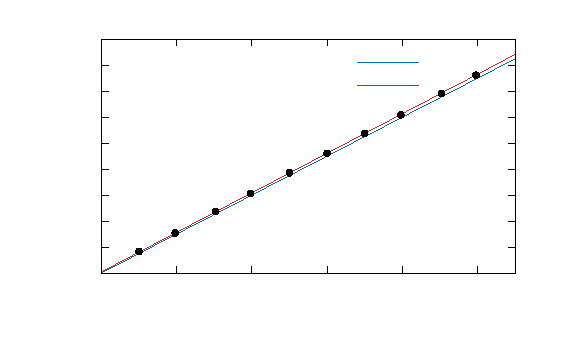
\includegraphics[width={259.10bp},height={158.40bp}]{neinvertujici}}%
    \gplfronttext
  \end{picture}%
\endgroup
 }
        \captionsetup{type=graph}
        \caption{Závislost výstupního napětí na vstupním při zapojení s neinvertujícím vstupem}
    \end{minipage} 
\end{table}

\newpage

\subsection{Rozdílový zesilovač}

Kombinací invertujícího a neinvertujícího zesilovače jde vytvořit rozdílový zesilovač uvedený na obrázku 6. Pro jeho výstupní napětí platí vztah

\begin{equation}
    U_0 = U_2 \frac{R_4 (R_1 + R_2)}{R_1 (R_3 + R_4)} - U_1 \frac{R_2}{R_1}.
\end{equation}

\begin{figure}[h]
    \centering
    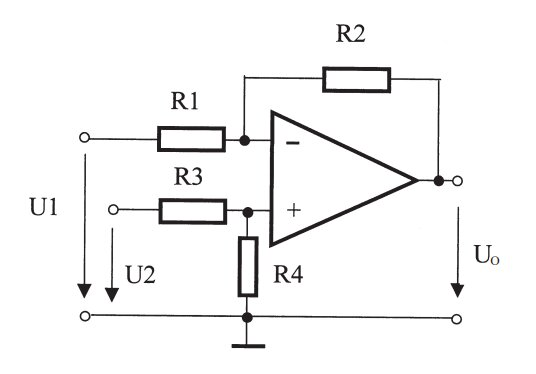
\includegraphics[width=0.4\textwidth]{rozdilovy_sch.jpg}
    \caption{Rozdílový zesilovač}
\end{figure}

Velikost rezistorů zvolím $ R_1 = R_3 = 10 \text{ k} \Omega $ a $ R_2 = R_4 = 20 \text{ k}\Omega $, čímž se vztah (6) zjednoduší na tvar $ U_0 = 2(U_2 - U_1) $. Naměřená data jsou v tabulce 5 a z fitu přímkou vyšlo zesílení

\begin{equation}
\frac{U_0}{U_2 - U_1} =  2.028 \pm 0.002 
\end{equation}

\begin{table}[h]
    \begin{minipage}[b]{.45\linewidth}
        \centering
        \begin{tabular}{ | c c c c | }
            \hline
            $ U_1 $ (V) & $ U_2 $ (V) & $ U_0 $ (V) & $ U_0 $ (V) teoretická\\
            \hline
            1.49 & 1.26 & -0.46 & -0.46 \\
            1.49 & 1.49 & 0.00  & 0.00   \\
            1.49 & 2.00 & 1.04  & 1.02 \\
            1.49 & 2.24 & 1.52  & 1.50  \\
            1.49 & 2.50 & 2.04  & 2.02 \\
            1.49 & 2.75 & 2.56  & 2.52 \\
            1.49 & 2.97 & 3.02  & 2.96 \\
            1.49 & 3.25 & 3.57  & 3.52 \\
            1.49 & 3.50 & 4.08  & 4.02 \\
            1.49 & 3.74 & 4.57  & 4.50  \\
            1.49 & 4.00 & 5.08  & 5.02 \\
            2.05 & 1.50 & -1.09 & -1.1 \\
            2.05 & 1.75 & -0.60 & -0.6 \\
            \hline
        \end{tabular}
        \caption{Naměřená vstupní a výstupní napětí}
    \end{minipage} 
    \hfill
    \begin{minipage}[b]{.45\linewidth}
        \centering
        \resizebox{\textwidth}{!}{ % GNUPLOT: LaTeX picture with Postscript
\begingroup
  \makeatletter
  \providecommand\color[2][]{%
    \GenericError{(gnuplot) \space\space\space\@spaces}{%
      Package color not loaded in conjunction with
      terminal option `colourtext'%
    }{See the gnuplot documentation for explanation.%
    }{Either use 'blacktext' in gnuplot or load the package
      color.sty in LaTeX.}%
    \renewcommand\color[2][]{}%
  }%
  \providecommand\includegraphics[2][]{%
    \GenericError{(gnuplot) \space\space\space\@spaces}{%
      Package graphicx or graphics not loaded%
    }{See the gnuplot documentation for explanation.%
    }{The gnuplot epslatex terminal needs graphicx.sty or graphics.sty.}%
    \renewcommand\includegraphics[2][]{}%
  }%
  \providecommand\rotatebox[2]{#2}%
  \@ifundefined{ifGPcolor}{%
    \newif\ifGPcolor
    \GPcolorfalse
  }{}%
  \@ifundefined{ifGPblacktext}{%
    \newif\ifGPblacktext
    \GPblacktexttrue
  }{}%
  % define a \g@addto@macro without @ in the name:
  \let\gplgaddtomacro\g@addto@macro
  % define empty templates for all commands taking text:
  \gdef\gplbacktext{}%
  \gdef\gplfronttext{}%
  \makeatother
  \ifGPblacktext
    % no textcolor at all
    \def\colorrgb#1{}%
    \def\colorgray#1{}%
  \else
    % gray or color?
    \ifGPcolor
      \def\colorrgb#1{\color[rgb]{#1}}%
      \def\colorgray#1{\color[gray]{#1}}%
      \expandafter\def\csname LTw\endcsname{\color{white}}%
      \expandafter\def\csname LTb\endcsname{\color{black}}%
      \expandafter\def\csname LTa\endcsname{\color{black}}%
      \expandafter\def\csname LT0\endcsname{\color[rgb]{1,0,0}}%
      \expandafter\def\csname LT1\endcsname{\color[rgb]{0,1,0}}%
      \expandafter\def\csname LT2\endcsname{\color[rgb]{0,0,1}}%
      \expandafter\def\csname LT3\endcsname{\color[rgb]{1,0,1}}%
      \expandafter\def\csname LT4\endcsname{\color[rgb]{0,1,1}}%
      \expandafter\def\csname LT5\endcsname{\color[rgb]{1,1,0}}%
      \expandafter\def\csname LT6\endcsname{\color[rgb]{0,0,0}}%
      \expandafter\def\csname LT7\endcsname{\color[rgb]{1,0.3,0}}%
      \expandafter\def\csname LT8\endcsname{\color[rgb]{0.5,0.5,0.5}}%
    \else
      % gray
      \def\colorrgb#1{\color{black}}%
      \def\colorgray#1{\color[gray]{#1}}%
      \expandafter\def\csname LTw\endcsname{\color{white}}%
      \expandafter\def\csname LTb\endcsname{\color{black}}%
      \expandafter\def\csname LTa\endcsname{\color{black}}%
      \expandafter\def\csname LT0\endcsname{\color{black}}%
      \expandafter\def\csname LT1\endcsname{\color{black}}%
      \expandafter\def\csname LT2\endcsname{\color{black}}%
      \expandafter\def\csname LT3\endcsname{\color{black}}%
      \expandafter\def\csname LT4\endcsname{\color{black}}%
      \expandafter\def\csname LT5\endcsname{\color{black}}%
      \expandafter\def\csname LT6\endcsname{\color{black}}%
      \expandafter\def\csname LT7\endcsname{\color{black}}%
      \expandafter\def\csname LT8\endcsname{\color{black}}%
    \fi
  \fi
    \setlength{\unitlength}{0.0500bp}%
    \ifx\gptboxheight\undefined%
      \newlength{\gptboxheight}%
      \newlength{\gptboxwidth}%
      \newsavebox{\gptboxtext}%
    \fi%
    \setlength{\fboxrule}{0.5pt}%
    \setlength{\fboxsep}{1pt}%
    \definecolor{tbcol}{rgb}{1,1,1}%
\begin{picture}(4608.00,3600.00)%
    \gplgaddtomacro\gplbacktext{%
      \csname LTb\endcsname%%
      \put(682,704){\makebox(0,0)[r]{\strut{}$-2$}}%
      \put(682,1001){\makebox(0,0)[r]{\strut{}$-1$}}%
      \put(682,1298){\makebox(0,0)[r]{\strut{}$0$}}%
      \put(682,1596){\makebox(0,0)[r]{\strut{}$1$}}%
      \put(682,1893){\makebox(0,0)[r]{\strut{}$2$}}%
      \put(682,2190){\makebox(0,0)[r]{\strut{}$3$}}%
      \put(682,2487){\makebox(0,0)[r]{\strut{}$4$}}%
      \put(682,2785){\makebox(0,0)[r]{\strut{}$5$}}%
      \put(682,3082){\makebox(0,0)[r]{\strut{}$6$}}%
      \put(682,3379){\makebox(0,0)[r]{\strut{}$7$}}%
      \put(814,484){\makebox(0,0){\strut{}$-1$}}%
      \put(1239,484){\makebox(0,0){\strut{}$-0.5$}}%
      \put(1663,484){\makebox(0,0){\strut{}$0$}}%
      \put(2088,484){\makebox(0,0){\strut{}$0.5$}}%
      \put(2513,484){\makebox(0,0){\strut{}$1$}}%
      \put(2937,484){\makebox(0,0){\strut{}$1.5$}}%
      \put(3362,484){\makebox(0,0){\strut{}$2$}}%
      \put(3786,484){\makebox(0,0){\strut{}$2.5$}}%
      \put(4211,484){\makebox(0,0){\strut{}$3$}}%
    }%
    \gplgaddtomacro\gplfronttext{%
      \csname LTb\endcsname%%
      \put(209,2041){\rotatebox{-270}{\makebox(0,0){\strut{}$ U_0 $ (V)}}}%
      \put(2512,154){\makebox(0,0){\strut{}$ U_2 - U_1 $ (V)}}%
      \csname LTb\endcsname%%
      \put(3224,3206){\makebox(0,0)[r]{\strut{} teoretická závislost $2x$}}%
      \csname LTb\endcsname%%
      \put(3224,2986){\makebox(0,0)[r]{\strut{}fit}}%
    }%
    \gplbacktext
    \put(0,0){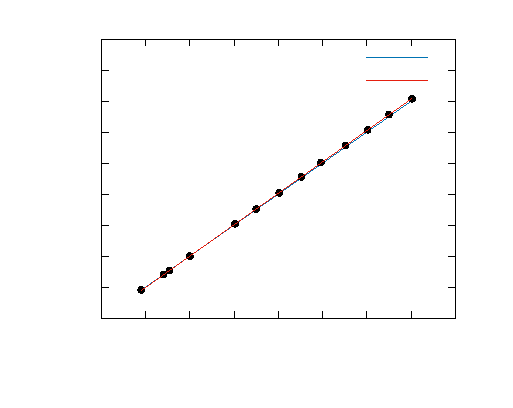
\includegraphics[width={230.40bp},height={180.00bp}]{rozdilovy}}%
    \gplfronttext
  \end{picture}%
\endgroup
 }
        \captionsetup{type=graph}
        \caption{Závislost výstupního napětí na vstupních rozdílu napětí.}
    \end{minipage} 
\end{table}

\newpage

\subsection{Derivátor}

Derivátor je zapojení, které by mělo na výstupu $ U_0 $ udávat derivaci vstupního napětí $ U_1 $. Je stejné jako zapojení s invertujícím vstupem, s rozdílem, že jeden odpor je nahrazený kondenzátorem. Proud jím tekoucí je přímo úměrný derivaci napětí na něm, a protože oběma větvemi teče stejný proud, máme

\begin{equation}
U_0 = - \frac{R}{C} \dot U_1
\end{equation}


\begin{figure}[htpb]
    \centering
    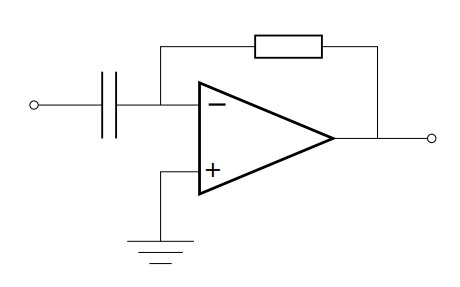
\includegraphics[width=0.4\textwidth]{derivator_sch.jpg}
    \caption{Zapojení zesilovače jako derivátoru}
\end{figure}


Na vstupním napětí jsem nastavil sinusový signál $ \sin(x) $  a na výstupu pozoroval $ - \cos(x) $, jak to předpovídá vztah (8). Druhým testem bylo vstupní napětí ve tvaru pily, kde na výstupu byly vidět obdélníkové pulzy. 

\section{Závěr}

V této úloze jsem ověřil základní vlastnosti operačního zesilovače. U zapojení komparátoru jsem pozoroval očekávané přepínání polarity výstupního napětí v závislosti na rozdílu vstupních hodnot $U_1$ a $U_\text{ref}$ a při zapojení s invertujícím a neinvertujícím vstupem jsem získal zesílení $-2.033 \pm 0.001$ a $ 3.045 \pm 0.002 $, což bylo v dobré shodě s předpokládanou hodnotou $ -2 $ a $ 3 $.

Šířku pásma zesilovače jsem určil do $40 $ kHz při zapojení s invertujícím vstupem a zjistil, že se toto rozmezí dá rozšířit zapojením paralelního kondenzátoru do zpětnovazební větve u tzv. dolnofrekvenční propusti, kdy se šířka zvětšila na $ 168 $  kHz, při kapacitě kondenzátoru $ 10 $ nF.

Dalším úkolem bylo zapojení rozdílového zesilovače, kde jsem na výstupu pozoroval zesílení rozdílu vstupních napětí o $ 2.028 \pm 0.002 $, když předpokládaná hodnota měla být $ 2 $.

Dobře fungovalo i zapojení derivátoru, kde jsem na výstupu pozoroval časovou derivaci napětí na vstupu. 



\begin{thebibliography}{0}
\bibitem{tabulky} Návod k úloze ~\url{}.   
\end{thebibliography}

\end{document}
